\documentclass[a4paper]{article}
\usepackage[a4paper, left=25mm, right=25mm, top=25mm, bottom=25mm]{geometry}
%\geometry{paperwidth=210mm, paperheight=2000pt, left=5pt, top=5pt}
\usepackage[utf8]{inputenc}
\usepackage[english,russian]{babel}
\usepackage{indentfirst}
\usepackage{tikz} %Рисование автоматов
\usetikzlibrary{automata,positioning,arrows,trees}
\usepackage{amsmath}
\usepackage{enumerate}
\usepackage[makeroom]{cancel} % зачеркивание
\usepackage{multicol,multirow} %Несколько колонок
\usepackage{hyperref}
\usepackage{tabularx}
\usepackage{amsfonts}
\usepackage{amssymb}
\usepackage{amsmath}
\DeclareMathOperator{\Tr}{Tr}
\DeclareMathOperator{\diag}{diag}
\DeclareMathOperator{\conv}{conv}
\DeclareMathOperator{\Rg}{Rg}
\DeclareMathOperator{\Ker}{Ker}
\newcommand{\matrixl}{\left|\left|}
\newcommand{\cbad}{c_{\mathrm{bad}}}
\newcommand{\matrixr}{\right|\right|}
\DeclareMathOperator*{\argmin}{arg\,min}
\usepackage{wasysym}
\date{\today}
\title{On the feasibility for the system of quadratic equations.\\Minimizing $z(c)$ when $|\cbad|=\infty$}

\begin{document}
\maketitle
\section{The framework}
In this section, the framework for finding convex cuts is described. We start from the definition of a quadratic map, then the task is set formally and then is formulated as a constrainted optimization problem.

Let $f\colon\mathbb{R}^n\to\mathbb{R}^m$ be a quadratic map: $f_i(x)=x^TA_ix+2b_i^Tx$, $A_i^T=A_i$. We want to explore the image $F=f(\mathbb{R}^n)$ and find convex parts of $F$.
\begin{enumerate}
\item Consider a problem
\begin{equation}
\label{min} g(c)=\min\limits_{x\in\mathbb{R}^n}(c,f(x))
\end{equation}

It has a finite solution iff \ref{minimum}

$$
\begin{cases}c\cdot A\geqslant0\\
(c\cdot b)^T\Ker (c\cdot A)=0\end{cases}
$$


The $x$, minimizing \ref{min} are ($Q^g$ is a pseudoinverse of $Q$)
$$x=\Ker(c\cdot A)-(c\cdot A)^g(c\cdot b)$$

This way, we found pre-images $X(c)$ of boundary points of $F$ lying on the supporting hyperplane with a normal vector $c$:

$$X(c)=\argmin (c, f(x))=\Ker(c\cdot A)-(c\cdot A)^g(c\cdot b)$$

\item Let $c_+$ be a vector from $\mathbb{R}^m$ s.t. $c_+\cdot A>0$. Then the supporting hyperplane with the normal vector $c_+$ is touching $F$ at a single point $y_0=f(x_0)$, where $$x_0=-(c_+\cdot A)^{-1}(c_+\cdot b)$$


We want to find the maximum value $z_{\max}$ such that $Z\subseteq F$ is convex:
$$Z=\{y\big| (c_+,y-y_0)\in[0,z_{\max}]\}$$

To do that, we find c such that set $f(X(c))$ is nonconvex, project points of $f(X(c))$ to $c_+$ and find a minimum of the projection:

\begin{equation}
\label{zc}
z_{\max}=\inf_c \tilde{z}(c),\, \tilde{z}(c)=\inf \big(c_+, f(X(c))-f(x_0)\big)
\end{equation}


\item To find $\tilde{z}(c)=\inf\limits_{x\in \Ker(c\cdot A)-(c\cdot A)^g(c\cdot b)}(c_+,f(x)-f(x_0))$, we introduce the plus norm in the $q\in\mathbb{R}^n$ space
$$||q||^2_+=q^T(c_+\cdot A)q$$

Note that \ref{norm} $(c_+,f(x)-f(x_0))=||x-x_0||_+^2$.
Therefore, $\tilde{z}(c)=\rho_+^2(\Ker(c\cdot A)-(c\cdot A)^g(c\cdot b),x_0)$
\item Next, we change variables to find $\tilde{z}(c)$ explicitly. We use the following change
$\begin{cases}
x=S\hat{x}+x^0\\
y=\hat{y}+y^0
\end{cases}$ $y=f(x)$, $\hat{y}=\hat{f}(\hat{x})$ and demand $\begin{cases}
c_+\cdot A=I\\
c_+\cdot b=0
\end{cases}$. It leads \ref{variables} to
$$x^0=x_0,\,y^0=y_0,\,S=S_1S_2,\, S_1^T(c_+\cdot A)S_1=\Lambda,\,S_1^TS_1=I,\,S_2=\Lambda^{-1/2},\,\begin{cases}
\hat{A}_i=S^TA_iS\\
\hat{b}_i=S^T(b_i+A_ix^0)
\end{cases}$$

In new variables $||\hat{q}||_+^2=\hat{q}^T\hat{q}$, i.e. the new basis is orthonormal w.r.t. $||\cdot||_+$, because $c_+\cdot A=I$.


Notice that $\tilde{z}(c)=\rho_+^2(x_0,\Ker (c\cdot A)-(c\cdot A)^g(c\cdot b))=\mathrm{diam}(\Ker(c\cdot \hat{A})-(c\cdot \hat{A})^g(c\cdot \hat{b}))=||(c\cdot A)^g(c\cdot b)||^2$ since $\Ker(c\cdot \hat{A})^T\big((c\cdot A)^g(c\cdot b)\big)=0$ \ref{minimum}

\item We associate the condition $\Rg(c\cdot A)\leqslant n-1$, $c\cdot A\geqslant 0$ with nonconvexity of $f(X(c))$. The real sufficient condition for nonconvexity is given by the Theorem 3.4, which requires some additional constraints on $c$:
$$
\begin{cases}
Rg(c\cdot A)=n-1\\
f^1\nparallel f^2
\end{cases}
$$
But we assume that other cases, in particular, $Rg(c\cdot A)<n-1$ or $f^1\parallel f^2$ are rare.

\item Let us note that if $f(X(c))$ is nonconvex, then $\lambda_{\min}(c\cdot A)=0$. Consider $\tilde{z}(c+\alpha c_+)=||(c\cdot A+\alpha I)^g(c\cdot b)||^2$, since $c_+\cdot\hat{A}=I,\,c_+\cdot\hat{b}=0$. Therefore, adding $\alpha c_+$ to $c$ adjusts the spectrum of $c\cdot A$. If and only of we choose $\alpha=-\lambda_{\min}(c\cdot A)$, $\tilde{z}$ will be associated with a $\tilde{c}=c+\alpha c_+$ for which $\lambda_{\min}(\tilde{c}\cdot A)=0$. This way, for every given $c\in\mathbb{R}^m$ we can find one and only one $\tilde{c}=c+\alpha c_+$ such that $\lambda_{\min}(\tilde{c}\cdot A)=0$

We define $z(c)=||\big((c\cdot \hat{A})-\lambda_{\min}(c\cdot \hat{A})\big)(c\cdot \hat{b})||^2$, which is the same as $\tilde{z}(c-\lambda_{\min}c_+)$. This way, we automatically choose the adjustment to the spectrum to ensure that $\lambda_{\min}(c\cdot A-\lambda_{\min}(c\cdot A))=0$

Notice that $z(c+\mu c_+)=z(c)$.

\item Next, we define $Q(c)=c\cdot \hat{A}-\lambda_{\min}(c\cdot \hat{A})$, $\hat{b}_c=c\cdot \hat{b}$, $v(c)=Q(c)^gb_c$. Then $$z(c)=||v(c)||^2=v^Tv$$

Note that $z(c)$ has its geometrical meaning \ref{zc} only if $c\in\cbad=\{c\big|\Ker Q(c)\bot b_c\}$.
\end{enumerate}

At this point, we have a function $z(c)$ defined on $\cbad$ and we want to minimize it. We assume that it is continuous and differentiable, and also that $\cbad$ contains connected parts (manifolds)

\section{Minimization}
In this section we address the problem of finding minimum of $z(c)$ stated in the previous section. Again, we assume that $\cbad$ contains a manifold and we have a point $c$ in it already. We use well-known techique, Gradient projection method to solve it. We use not the Euclidean projection, but a very special one based on the geometry of $\cbad$. The method's two steps, gradient step and projection, are discussed in details below.

Formally, we want to find
\begin{equation}
z_{\max}=\inf\limits_{c\in\cbad}z(c)
\end{equation}

Let $\pi_{\cbad}$ be an operator which projects a point onto $\cbad$. Then the method is the following:
$$c^{(k+1)}=\underbrace{\pi_{\cbad}}_{\mathrm{proj.}}(\underbrace{c^{(k)}-\beta^k \nabla z(c^{(k)})}_{\mathrm{gradient \,\,step}})$$


Nonconvexity certificate gives a single point $c\in \cbad$, which is used as a start point $c^{(1)}$. We assume $\Rg Q(c)=n-1$

Define $k(c)\in\mathbb{R}^n$ s.t. $k(c)\in\Ker Q(c)$, $||k(c)||=1$. We assume that for any $c'$ the dot product $k(c')^Tk(c)>0$ (change sign if false).
Each iteration has two key elements: gradient step and projection (see image below)

Assume that we have done $k-1$ steps already and obtained a point $c=c^{(k)}$. The next two sections describe how to obtain the next point $\tilde{c}=c^{(k+1)}$.

\subsection{Gradient step}
Define $R_i=\hat{A}_i-k^T\hat{A}_ik$, $q_i=\hat{b}_i-R_iv$. Then \ref{gradient}
$$\nabla_iz\equiv \frac{\partial z}{\partial c_i}=2v^TQ^gq_i$$

Define $n_i=k^Tq_i$. Then $n$ is a normal vector to $\cbad$ at a point $c$ (see picture). We eliminate normal part of the gradient to decrease the distance to $\cbad$ (see picture):
$$c'=c-\beta\left(I-n\frac{(\cdot, n)}{|n|^2}\right)\nabla z$$

\subsection{Projection}
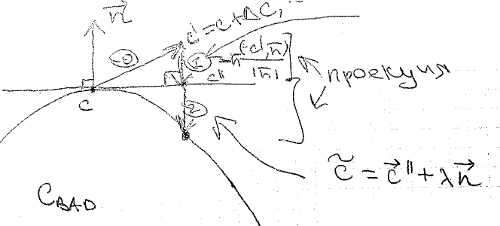
\includegraphics[width=0.8\textwidth]{c_bad_continuum.png}

We next assume that for some $\lambda\in\mathbb{R}$ vector $\tilde{c}(\lambda)=c'+\lambda n\in\cbad$. To find $\lambda$, we write the condition $\tilde{c}\in\cbad\Leftrightarrow (\tilde{c}\cdot \tilde{b})^T k(\tilde{c}(\lambda))=0$. We define a function
$$m(\lambda)=(\tilde{c}(\lambda)\cdot \tilde{b})^T k(\tilde{c}(\lambda))$$

This function is continuous if $\Rg Q(\lambda)=n-1$ in the neighbourhood of $\lambda$. Next, we find its root using bisection method on $[-\lambda_0,\lambda_0]$, $\lambda_0=||c-c'||$.

For some $\lambda$, $m(\lambda)=0$ means that $\tilde{c}=c'+\lambda n\in\cbad$, and that the projection step was a success.

If the method does not converge on the interval given, or rank problem ($\Rg Q\neq n-1$) occurs, we reduce the gradient step $\beta\to \theta\beta$, $\theta <1$, recalculate $c'$ and try the projection again.

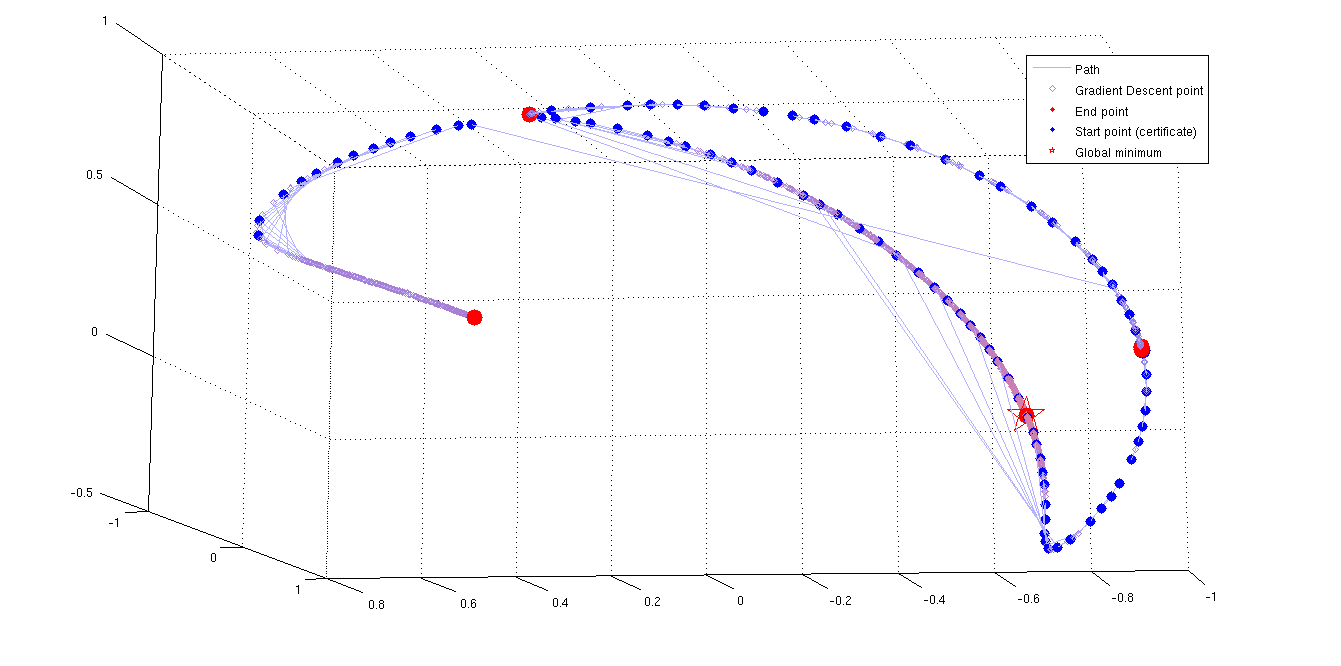
\includegraphics[width=0.7\textwidth]{example03_cbad_91pts_04.png}

This way, we can construct a new point $\tilde{c}$ from the previous one $c$, and $\tilde{c}$ has lower value of $z(\cdot)$. We continue until the Gradient projection method condition holds:
$$\nabla z|| n$$

If this condition holds, then the resulting $\tilde{c}$ is the same as $c$ on previous iteration, and the iterations stop.

\section{Explanations}
This section contains explanations and proofs for the main article and draft.pdf.
\subsection{$F$ and $\conv F$}
Consider $f\colon \mathbb{R}^n\to\mathbb{R}^m$, s.t. $f_i(x)=x^TA_ix+2b_i^Tx$, $A_i=A_i^T$. Define $F=f(\mathbb{R}^n)$.

Then why $A=\inf \limits_{y\in F} (c,y)=\inf\limits_{y\in\conv F} (c,y)=B$?

\begin{enumerate}
\item First, $F\subseteq \conv F$, therefore, $B\leqslant A$.
\item Secondly, let $y_k\in \conv F$ be a sequence s.t. $g_k=(c,y_k)\underset{k\to\infty}{\longrightarrow} B$. $y_k=\sum\limits_{i=1}^{n_k}\alpha^k_iy^k_i$.

$g_k(c,y_k)=\sum\limits_{i=1}^{n_k}\alpha^k_i(c,y^k_i)=\sum\limits_{i=1}^{n_k}\alpha^k_i g^k_i$. Define $g^k_0=\min\limits_{i\in \overline{1,n_k}}g^k_i$. Then $B\leqslant g^k_0\leqslant g^k$. Therefore, $g^k_0\to B$ also. This way, we have constructed a sequence $y^k_0\in F$ s.t. $(c,y^k_0)\to B$, therefore, $A\leqslant B$.
\end{enumerate}

\subsection{Minimum of $f(x)$} \label{minimum}
Consider $f\colon \mathbb{R}^n\to\mathbb{R}^m$. $f_i(x)=x^TA_ix+2b_i^Tx$. $A_i^T=A_i$. Let $c\in\mathbb{R}^m$

We want to find
$g(c)=\inf\limits_{x\in\mathbb{R}^n} (c,f(x))$.

Define $A_c\equiv c\cdot A=\sum\limits_{i=1}^m c_iA_i$, $b_c=c\cdot b=\sum\limits_{i=1}^m c_ib_i$.

$(c,f(x))=\sum\limits_{i=1}^m c_i f_i(x)=\sum c_i (x^TA_ix+2b_i^Tx)=x^TA_cx+2b_c^Tx$.

If $\exists v\colon -\alpha=v^TA_cv<0$ then $g(c)=-\infty$:
$g(\beta v)=-\beta^2\alpha+\beta 2b_c^Tv\to-\infty,\,\beta\to+\infty$.

From this point on, we assume $A_c\geqslant 0$. Let $R_0$ be a zero eigenspace (=kernel) of $A_c$: $R_0=\{v\colon A_cv=0\}=\ker A_c$

If $\exists v\in R_0\colon v^Tb_c\neq 0$ then $g(c)=-\infty$: Consider $f(\beta v)=\beta^2 v^T\cancelto{0}{(A_cv)}+2\beta \underbrace{b_c^Tv}_{\neq 0}\to-\infty,\, \beta\to\infty$

Then $R_0\subseteq \{b_c\}^\bot$

Consider $A=\sum\limits_{i=1}^n \lambda_i s_is_i^T=S\Lambda S^T$, $S=||s_1 ... s_n ||$, $S^TS=E$, $s_i^Ts_j=\delta_{ij}$.

$f$ is differentiable, then for finding $g(c)$ the gradiend $\nabla (c,f(x))=2A_cx+2b_c=0$.

$$S\Lambda S^Tx=-b_c\Leftrightarrow \Lambda S^Tx=-S^Tb_c\, (*)$$.

Let $x$ be $x=x^{\parallel}+x^\bot$, $x^{\parallel}\in R_0$, $x^\bot \bot R_0$.

Then neither $f(x)$ nor $\Lambda S^T x$ depend on $x^{\parallel}$. This means that the $x$ minimizing $g(c)$ is defined in terms of $x^{\bot}$ and $x^{\parallel}$ is arbitrary.

Define $\lambda^g_i=\begin{cases}
0,&\lambda_i=0\\
1/\lambda_i,&\lambda_i\neq 0
\end{cases}$. Define $\Lambda^g=\diag(\lambda^g_1,...,\lambda^g_n)$. Then $\Lambda \Lambda^g=\delta_{ij}[\lambda_i\neq 0]$. Then $S\Lambda^g\Lambda S^T$ is a projector on $R_0^\bot$.

Consider $(*) \Leftrightarrow \Lambda^g\Lambda S^T(x^\parallel+x^\bot)=-\Lambda^gS^Tb_c$. But $\Lambda S^Tx^\parallel=0$, therefore, $\underbrace{S\Lambda^g\Lambda S^T}_{\mbox{\tiny projector}}x^\bot=-S\Lambda^gS^Tb_c$. But $x^\bot$ is already in $R_0^\bot$, therefore, $x^\bot=-\underbrace{S\Lambda^gS^T}_{A^g_c}b_c$. Here $A_c^g$ is a pseudoinverse of $A_c$.

Therefore, $\boxed{x=-A_c^gb_c+x^\parallel}$, where $x^\parallel\in R_0$.

%Let us notice that since $A_c^{gT}=A_c^g$

Consider $(c,f(x))=(c,f(x^\bot))=b_c^TA_c^gA_cA_c^gb_c-2b_c^TA_c^gb_c$. Consider $A_cA_c^gb_c=S\Lambda \cancelto{E}{S^TS}\Lambda^gS^Tb_c$. Because $R_0\subseteq\{b_c\}^\bot$, $\Lambda\Lambda^gS^Tb_c=S^Tb_c$. Therefore, $A_cA_c^gb_c=b_c$. Then $(c,f(x))=b_c^TA_c^gb_c-2b_c^TA_c^gb_c=\boxed{-b_c^TA_c^gb_c}$

\subsection{Finding $c$ provided $d$}
Let $H\colon \mathbb{R}^{n+1, n+1}\to \mathbb{R}^n$ be a map s.t. $H_i(X)=\Tr(H_iX)$, $$H_i=\left|\left|
\begin{array}{cc}
A_i & b_i\\
b_i^T & 0
\end{array}
\right|\right|^{\Box}$$.

Consider a boundary point $X$, which is a solution of (main article, (4)):
$$\boxed{\sup\limits_{\begin{cases}
H(X)=y^0+td\\
X\geqslant 0\\
X_{n+1,n+1}=1
	\end{cases}} t}$$

Define $f(t,X)=t$, $D_0=\{(t,X)\big| X\geqslant 0,\, X_{n+1,n+1}=1 \}$, $D_1=\{(t,X)\big| H(X)=y^0+td\}$.

Then supremum is equivalent to

$$\sup\limits_{(t,X)\in D_0\cap D_1}f(t,X)$$

Define a Lagrange function $L(c,t,X)=\underbrace{t}_{f(t,X)}+\sum\limits_{i=1}^m c_i(y^0_i+td_i-H_i(X))$.

Here we divided the constraints into two parts: $D_1$ goes to the Lagrange function, $D_0$ goes to the inner supremum. {\em Stephen Boyd, Lieven Vandenberghe. Convex Optimization. Page ???. Cambridge University Press}

Then the dual function is $g(c)=\sup\limits_{(t,X)\in D_0} L(c,t,X)$.

Because $L=t(1+\sum\limits_{i=1}^m c_id_i)+\sum\limits_{i=1}^n c_i(y^0_i-H_i(X))$, $g=+\infty$ when $(c,d)\neq -1$. From this point we assume that $\boxed{(c,d)=-1}$.

Now, $g(c)=\sup\limits_{X_{n+1,n+1}=1,X\geqslant 0} (c,y^0-H(X))=(c,y^0)+\sup\limits_{y\in\conv F} -(c,y)=(c,y^0)-\inf\limits_{y\in\conv F} (c,y)$.

Then the dual problem is
$$g(c)\to\inf\limits_{(c,d)=-1}$$

Let us prove that $\inf\limits_{y\in\conv F} (c,y)=\inf\limits_{H=\left|\left|
\begin{array}{cc}
A_c & b_c\\
b_c^T&\gamma
\end{array}
\right|\right|\geqslant 0}(-\gamma)$

Via Schur complement $H\geqslant 0\Leftrightarrow \begin{cases}
A_c\geqslant 0\\
\gamma-b_c^TA_c^gb_c\geqslant 0\\
(E-A_cA_c^g)b_c=0
\end{cases}$.

$A_c\geqslant 0$ is a necessary condition for $\exists g(c) \in\mathbb{R}$ (see part 2).

$(E-A_cA_c^g)b_c=0$ is another necessary condition for $\exists g(c)\in\mathbb{R}$.

Statement $\gamma\geqslant b_c^TA_cb_c$ means $-\gamma\leqslant -b_c^TA_cb_c=\inf\limits_{y\in\conv F}(c,y)$, which means that $-\gamma$ is a lower bound for $\inf\limits_{y\in\conv F}(c,y)$.

Then $H\geqslant 0\Leftrightarrow -\gamma\leqslant \inf\limits_{y\in\conv F}(c,y)$.

Then $g(c)=(c,y^0)-\inf\limits_{H\geqslant 0}{-\gamma}$.

Then the dual problem is:

$\inf\limits_{(c,d)=-1}g(c)\Leftrightarrow \inf\limits_{(c,d)=-1}\left[(c,y^0)-\inf\limits_{H\geqslant 0}(-\gamma)\right]\Leftrightarrow \inf\limits_{(c,d)=-1}\inf\limits_{H\geqslant 0}(c,y^0)+\gamma=\boxed{\inf\limits_{\begin{cases}
H\geqslant 0\\
(c,d)=-1
\end{cases}}\gamma+(c,y^0)}$.

This problem is exactly (5) from main article $\blacksquare$.

\subsection{What is $z_{\max}$?}
\label{norm}
Consider $f\colon\mathbb{R}^n\to\mathbb{R}^m$, $f_i(x)=x^TA_ix+2b_i^Tx$, $A_i=A_i^T$.

Let $c_+\in\mathbb{R}^m$ s.t. $A_+=\sum c_iA_i > 0$. Then the minimum $\inf\limits_x (c,f(x))$ is obtained at a single point $x_0=-A_+^{-1}b_+$, $b_+=\sum c_ib_i$.

Consider $S_\varepsilon^+=\{x\in\mathbb{R}^n\big| (x-x_0)^TA_+(x-x_0)= \varepsilon^2\}$. Then $f(S_\varepsilon^+)=\{y\in\mathbb{R}^m\big| (c_+,y)=(c_+,f(x_0))+\varepsilon^2 \}$.

Indeed, if $\begin{cases}
P=(c_+,f(x)-f(x_0))\\
Q=(x-x_0)^TA_+(x-x_0)
\end{cases}$
then $P-Q=\underline{x^TA_+x}-x_0^TA_+x_0+2b_+^Tx-2b_+^Tx_0-\underline{x^TA_+x}-x_0^TA_+x_0+2x^TA_+x_0=\left/x_0=-A_+^{-1}b_+\right/=2x_0^Tb_++2b_+^Tx-2b_+^Tx_0-2x^Tb_+=0$.

$\boxed{\mbox{{\bf Therefore, the image of $B_\varepsilon^+$ is a {\em convex cut}} $\{y\big| (c_+,y)\in (c_+,f(x_0))+[0,z_{\max}]\}$}}$

\subsection{Variables s.t. $c\cdot A=I,\,c\cdot b=0$}
\label{variables}
Given: the map $f\colon\mathbb{R}^n\to\mathbb{R}^m$, $f_i(x)=x^TA_ix+2b_i^Tx$, $A_i=A_i^T$, vector $c\in\mathbb{R}^m\colon c\cdot A>0$

We need to find a new pair of bases s.t. $\begin{cases}
\tilde{c}\cdot \hat{A}=I & (1)\\
\tilde{c}\cdot \hat{b}=0 & (2)
\end{cases}$

We choose $x=S\hat{x}+x^0$, $y=\hat{y}+y^0$, $f(x)=y$, $\hat{f}(\hat{x})=\hat{y}$.
Consider $f_i(x)=x^{0T}A_ix^0+\hat{x}^TS^TA_iS\hat{x}+2x^{0T}A_iS\hat{x}+2b_i^TS\hat{x}+2b_i^Tx^0=\hat{x}^T\underbrace{S^TA_iS}_{\hat{A}_i}\hat{x}+2\hat{x}^T\underbrace{S^T(b_i+A_ix^0)}_{\hat{b}_i}+\underbrace{x^{0T}A_ix^0+2b_i^Tx^0}_{y^0_i}$

$c\cdot \hat{A}=S^Tc\cdot AS=I$, then $S=S_1S_2$, $S_1^TA_iS_1=\Lambda=\diag$, $S_1^TS_1=I$, $S_2=\Lambda^{-1/2}$.

$c\cdot \hat{b}=S^T(c\cdot b+(c\cdot A)x^0)$. Then $x^0=-(c\cdot A)^{-1}(c\cdot b)$.

The algorithm:
\begin{enumerate}
\item Compute $S_1$ via the eigenbasis of $c\cdot A$, $S_1^T(c\cdot A)S_1=\Lambda$
\item Compute $S_2=\Lambda^{-1/2}$, $S=S_1S_2$.
\item Compute $x^0=-(c\cdot A)^{-1}(c\cdot b)$
\item Compute $\tilde{A}_i=S^TA_iS$, $\tilde{b}_i=S^T(b_i+A_ix^0)$
\end{enumerate}
\subsection{$z(c)=?$}
Given: the map $f\colon\mathbb{R}^n\to\mathbb{R}^m$, $f_i(x)=x^TA_ix+2b_i^Tx$, $A_i=A_i^T$, two vectors $c,c_+\in\mathbb{R}^m$. $c_+A=I$, $c_+b=0$.
Find: $z(c)=\inf\limits_{y\in Y} (c_+, y)$ where $Y$ is an intersection of $f(\mathbb{R}^n)$ with a tangent hyperplane defined by its normal vector $c$.

Define $\sigma(Q)=\{\lambda\big |\dim\Ker (Q-\lambda E)>0\}$. Define $\lambda_{\min}(Q)=\min\sigma(Q)$~--- minimal eigenvalue of $Q$.

\begin{enumerate}
\item If $\lambda_{\min}(c\cdot A)<0$ then the tangent hyperplane does not exist, and $z(c)=+\inf$
\item Then $\lambda_{\min}(c\cdot A)>0$, then there is no nonconvexity, and $z(c)=\inf$
\item For $\lambda_{\min}=0$ in part 2 $Y$ was found explicitly: $Y=\{f(x)\big|x=x^\parallel-A_c^gb_c, x^\parallel \in\Ker A_c\}$. Then for $y\in Y$ $(c_+,y)=x^T(\cancelto{I}{c_+\cdot A})x+2(\cancelto{0}{c_+\cdot b})^Tx=\boxed{x^Tx}$
\item $x^Tx=||x||^2=||x^\parallel||^2+||A_c^gb_c||^2$. We want to minimize $(c_+,y)$, therefore, we choose $x^\parallel=0$. Then $z(c)=||A_c^gb_c||^2=\boxed{\big|(c \cdot A)^g(c\cdot b) \big|^2}$
\item Consider $\inf\limits_{x\in\mathbb{R}^n} (c_+,f(x))=-(\cancelto{0}{c_+\cdot b})(\cancelto{I}{A_{c_+}})^{-1}(c_+\cdot b)=0$. Therore, $z(c)=\inf\limits_{y\in Y}(c_+,y)-\inf\limits_{y\in F}(c_+,y)$
\end{enumerate}

Now consider $z(c)=\begin{cases}
|(c\cdot A)^g(c\cdot b)|^2,&\lambda_{\min}(c\cdot A)=0\\
+\infty, & \mbox{otherwise}
\end{cases}$

Consider $z(c+\alpha c_+)=|(c\cdot A+\alpha \cancelto{I}{c_+\cdot A})^gb_c|^2=|(c\cdot A+\alpha I)^gb_c|^2$. We need $\alpha$ s.t. $\lambda_{\min}(c\cdot A+\alpha I)=0$, therefore, $\alpha=-\lambda_{\min}(c\cdot A)$.

Define $\hat{z}(c)=|(c\cdot A-\lambda_{\min}(A))^g(c\cdot b)|^2$. Consider $\mathbb{R}^m\ni c=c^{\parallel}+c^{\bot}$, $c^{\parallel}\parallel c_+$, $(c_+,c^{\bot})=0$.

Then $\hat{z}(c)=\hat{z}(c^{\bot})$, i.e. $\hat{z}$ does not depend on $c^{\parallel}$. It depends only on $c^{\bot}$, and $c^{\parallel}$ is chosen in a way that $\lambda_{\min}(c\cdot A)=0$.
\subsection{Theorem 3.4 (Nonconvexity certificate)}
Given.
\begin{enumerate}
\item The map $f\colon\mathbb{R}^n\to\mathbb{R}^m$, $f_i(x)=x^TA_ix+2b_i^Tx$, $A_i=A_i^T$, $m,n\geqslant 3$. The vector $c\in\mathbb{R}^m$.
\item $A_c\geqslant 0$, $\dim\Ker A_c=1$ (=simple zero eigenvalue), $\Ker A_c=\mbox{Lin}\{e\}$
\item $b_c\bot \Ker A_c$
\item $b\bot\Ker A_c$, $e^0=-A_c^gb_c$
\item $f(\alpha e+e^0)=f^0+2\alpha f^1+\alpha^2f^2$, $f^1\nparallel f^2$
\end{enumerate}
Then $F=\mbox{Im} f$ is nonconvex.

Consider $\inf\limits_{y\in F}(c,y)$ (part 2). $x=\underbrace{x^{\parallel}}_{\alpha e}+(\underbrace{-A_c^gb_c}_{e^0})$. Then

$$f_i(\alpha e + e^0)=\alpha^2 \underbrace{e^TA_ie}_{f^2_i}+2\alpha(\underbrace{b_i^Te+e^TA_ie^0}_{f^1_i})+\underbrace{2b_i^Te^0+e^{0T}A_ie^0}_{f^0_i}$$

If $f^1\nparallel f^2$, then $\{f(\alpha e+e^0\big| \alpha\in\mathbb{R})\}=F\cap \{y\big| (c,y)=\inf\limits_{y\in F} (c,y)\}$ is nonconvex. Then F is nonconvex.
\subsection{Equations (0.18)-(0.21)}
Consider $A(t)\colon n\times n$, $\exists \dot{A}$, $A^T=A$, $A\geqslant 0$, $A$ has a simple zero eigenvalue: $\forall t\,A(t)x_0(t)=0$, $x_0^Tx_0=0$.

Then $A=S\Lambda S^T$, $S^TS=E$, $A^g=S\Lambda^gS^T$. Define $\lambda_i=\Lambda_{ii}$. $\Lambda^g_{ii}=\begin{cases}
\frac{1}{\lambda_i},& \lambda_i\neq 0\\
0, &\lambda_i=0
\end{cases}$.

Then $AA^g=A^gA=S\Lambda S^TS\Lambda^gS^T=S\Lambda\Lambda^gS^T=\sum\limits_{\lambda_i\neq 0} s_is_i^T=1-x_0x_0^T$ (0.20)

Consider $\frac{d}{dt}Ax_0=\dot{A}x_0+A\dot{x}_0$. Multiplying by $A^g$ from the left: $A^g\dot{A}x_0+A^gA\dot{x}_0=0$.
Consider $A^gA\dot{x}_0=(1-x_0x_0^T)\dot{x}_0=\dot{x}_0-x_0x_0^T\dot{x}_0$. Since $||x_0||^2=x_0^Tx_0=1$, $x_0^T\dot{x}_0=0$. Then $-A^g\dot{A}x_0=\dot{x}_0$ (0.19).

Consider $\dot{A}x_0+A\dot{x}_0=0$. Multiplying by $x_0^T$ from the left: $x_0^T\dot{A}x_0+\cancelto{0}{x_0^TA}\dot{x}_0=0$. Then $x_0^T\dot{A}x_0=0$ (0.18)

Consider $AA^g=1-x_0x_0^T$. Then $\dot{A}A^g+A\dot{A}^g=-\dot{x}_0x_0^T-x_0\dot{x}_0^T=A^g\dot{A}x_0x_0^T+x_0x_0^T\dot{A}A^g$ (a)

Consider $A^gx_0=S\Lambda^gS^Tx_0=0$.

Multiplying (a) by $x_0$ from the right: $A\dot{A}^gx_0=A^g\dot{A}x_0$. Multiplying by $A^g$ from the left: $AA^g\dot{A}^gx_0=A^gA^g\dot{A}x_0$. Then $(1-x_0x_0^T)\dot{A}^gx_0=A^gA^g\dot{A}x_0$. Then $\dot{A}^gx_0=A^{-2}\dot{A}x_0+x_0x_0^T\dot{A}^gx_0$.

Let's multiply (a) by $A^g$ from the left: $A^g\dot{A}A^g+A^gA\dot{A}^g=A^{-2}\dot{A}x_0x_0^T+\cancelto{0}{A^gx_0}x_0^T\dot{A}A^g$.

Consider $A^gA\dot{A}^g=\dot{A}^g-x_0x_0^T\dot{A}^g=\dot{A}^g-x_0x_0^T\dot{A}A^{-2}-x_0x_0^T\dot{A}^gx_0x_0^T$.

Consider $x_0^T\dot{A}^gx_0=x_0^T(\dot{S}\Lambda^gS^T+S\dot{\Lambda^g}S^T+S\Lambda^g\dot{S}^T)x_0=x_0^T\dot{S}\Lambda^gS^Tx_0=0$.

Then $\frac{d}{dt}A^{-1}=-A^{-1}\dot{A}A^{-1}+x_0x_0^T\dot{A}A^{-2}+A^{-2}\dot{A}x_0x_0^T$ (0.21).

Case $\mbox{Rg}A<n-1$ is not considered since probability of such event is small.
\subsection{Gradient descent}
\label{gradient}
\begin{enumerate}
\item (0.5): $(\underbrace{c\cdot A-\lambda_{\min}(c\cdot A)}_Q)x_0=0$, then $\dot{x}_0=-Q^{-1}\dot{Q}x_0$. $\frac{d}{dt}\lambda_{\min}=\frac{d}{dt}x_0^T(c\cdot A)x_0=2\dot{x}_0\underbrace{(c\cdot A)x_0}_{\lambda_{\min}x_0}+x_0^T(\dot{c}\cdot A)x_0=2\lambda_{\min}\cancelto{0}{\dot{x}_0^Tx_0}+x_0^T(\dot{c}\cdot A)x_0$.

Then $\dot{x}_0=-(A_c-\lambda_{\min}(Ac))^{-1}(\dot{c}\cdot A-x_0^T(\dot{c}\cdot A)x_0)x_0$ (correct).
\item (0.6). $x_0^T(c\cdot b)=0$, use (0.5) (correct).
\item (0.7). $\frac{\partial}{\partial t}||v(c)||^2=\frac{\partial}{\partial t}\sum\limits_j v_j^2(c)=2\sum\limits_j v_j\frac{\partial}{\partial t}v_j=2v^T(c)\frac{d}{dt} v(c(t))$ (correct). $v(c)=(\underbrace{c\cdot A-\lambda_{\min}(c\cdot A}_Q)^{-1}(c\cdot b)=Q^{-1}(c\cdot b)$.
\item (0.8) Define $Q=c\cdot A-\lambda_{\min}(c\cdot A)$. Define $v=Q^{-1}(c\cdot b)$. Then $z(c)=||v||^2$ and $\dot{z}=2v^T\dot{v}$.

$\dot{v}=\dot{Q}^{-1}(c\cdot b)+Q^{-1}(\dot{c}\cdot b)$.

Consider (0.21) $\dot{Q}^{-1}=-Q^{-1}\dot{Q}Q^{-1}+x_0x_0^T\dot{Q}Q^{-2}+Q^{-2}\dot{Q}x_0x_0^T$.

Then $\dot{z}=2v^T\left(Q^{-1}(\dot{c}\cdot b)+(-Q^{-1}\dot{Q}Q^{-1}+x_0x_0^T\dot{Q}Q^{-2}+Q^{-2}\dot{Q}x_0x_0^T)(c\cdot b)\right)\boxed{=}$

$\boxed{=}2v^TQ^{-1}(\dot{c}\cdot b)-2v^TQ^{-1}\dot{Q}Q^{-1}(c\cdot b)+2\cancelto{0}{v^Tx_0}x_0^T\dot{Q}Q^{-2}(c\cdot b)+2v^TQ^{-2}\dot{Q}x_0\cancelto{0}{x_0^T(c\cdot b)}\boxed{=}$

Since $x_0\in \Ker Q\bot (c\cdot b)$, we have $x_0^T(c\cdot b)=0$.

Since $Qx_0=0$, $Q^{-1}x_0=0$: $Q^{-1}x_0=S\Lambda^{-1}S^Tx_0=S*0=0$. Since $v^T=(c\cdot b)^TQ^{-1}$. Then $v^Tx_0=0$

$\boxed{=}2v^TQ^{-1}(\dot{c}\cdot b)-2v^TQ^{-1}\dot{Q}\underbrace{Q^{-1}(c\cdot b)}_v=2v^TQ^{-1}(\dot{c}\cdot b)-2v^TQ^{-1}\dot{Q}v=\boxed{\dot{z}=2v^TQ^{-1}(\dot{c}\cdot b-\dot{Q}v)}$,

$\dot{Q}=\dot{c}\cdot A-x_0^T(\dot{c}\cdot A)x_0$

Since $\dot{z}=\sum \frac{\partial z}{\partial c_i}\frac{\partial c_i}{\partial t}$, $\frac{\partial z}{\partial c_i}$ can be found as a coefficient at $\dot{c}_i$ in $\dot{z}$

$\dot{z}=2v^TQ^{-1}\sum\limits_i\left(\dot{c}_ib_i-\dot{c}_iA_iv+x_0^T\dot{c}_iA_ix_0v\right)=\sum\limits_i \dot{c}_i\left[2v^TQ^{-1}(b_i-(A_i-x_0^TA_ix_0)v)\right]$

Thus, $\boxed{\frac{\partial z}{\partial c_i}=2v^TQ^{-1}(b_i-(A_i-x_0^TA_ix_0)v)}$, $Q=c\cdot A-\lambda_{\min}(c\cdot A)$, $v=Q^{-1}(c\cdot b)$, $x_0\in\Ker Q$, $||x_0||=1$

{\bf not the same as (0.8) in draft.pdf (but numerically same)}:

$\dot{z}_{(0.8)}=2\underbrace{(c\cdot b)^TQ^{-2}}_{v^TQ^{-1}}(\dot{c}\cdot b)-v^T(Q^{-1}\dot{Q}+\dot{Q}Q^{-1})v=2v^TQ^{-1}(\dot{c}\cdot b)-v^TQ^{-1}\dot{Q}v-v^T\dot{Q}Q^{-1}v$
\item (0.10). If $\dot{c}=\beta c_+$, then $\dot{z}=2v^TQ^{-1}(\dot{c}\cdot b-\dot{Q}v)=\boxed{=}$. Since $c_+\cdot b=0$, $c_+\cdot A=I$, $\dot{Q}=c_+\cdot A-x_0^T(c_+\cdot A)x_0=I-x_0^Tx_0=I-1=0$. And $\boxed{=}0$ (correct with new $\dot{z}$).
\item (0.14) $n_i=\left(b_i^T-v^T(A_i-x_0^TA_ix_0)\right)x_0$
\item (0.16) $P(\lambda)=Q^{-1}Q=S\Lambda^gS^TS\Lambda S^T=S\Lambda\Lambda^g S^T=1-x_0x_0^T$~--- projector on $(\Ker Q)^\bot$ (correct)
\item (0.15) $P(\lambda)(c(\lambda)\cdot b)=c(\lambda)\cdot b\Leftrightarrow \underbrace{(c(\lambda)\cdot b)\bot \Ker Q}_{\Leftrightarrow c(\lambda)\in c_{\mbox{\tiny bad}}}\Leftrightarrow c(\lambda)\cdot b\in\mbox{Im}Q\Leftrightarrow \exists \hat{x}\colon\, Q\hat{x}=c(\lambda)\cdot b$ (0.17) (correct)
\end{enumerate}
\subsection{Gradient descent. Projection}
We have $c\in\mathbb{R}^m$, $c\in c_{\mbox{\tiny bad}}=\{c\big| ||c||=1,\,\Ker Q(c)\bot (c\cdot b)\}$. $Q=c\cdot A-\lambda_{\min}(c\cdot A)$, $v=Q^{-1}(c\cdot b)$, $x_0\in\Ker Q$, $||x_0||=1$
\begin{enumerate}
\item Calculate $\frac{\partial z}{\partial c_i}=2v^TQ^{-1}(b_i-(A_i-x_0^TA_ix_0)v)$. Define $\Delta c=-\nabla z(c)$
\item Calculate $\hat{n}_i=\left(b_i^T-v^T(A_i-x_0^TA_ix_0)\right)x_0$, define $n_i=\frac{\hat{n}_i}{|\hat{n}|}$
\item Define $c'=c+\Delta c-n(\Delta c, n)$
\item Define $c(\lambda)=c'+\lambda n$. Define $x_0(\lambda)$ s.t. $x_0(\lambda)\in \Ker Q(\lambda)$, $x_0(\lambda)^Tx_0>0$, $||x_0(\lambda)||=1$. Define $m(\lambda)=(c(\lambda)\cdot b)^Tx_0(\lambda)$. Beware of $\mbox{Rg}Q<n-1$.
\item Find root of $m(\lambda)$ using binary search on $[-\lambda^0,\lambda^0]$, $\lambda^0=||c-c'||$.
\item Next $c$: $c(\lambda)$
\end{enumerate}

$m(\lambda)=0\Leftrightarrow (c(\lambda)\cdot b)\bot\{x_0\}=\Ker Q$ if $\mbox{Rg}Q=n-1$.
\subsection{Equation 0.19}
Consider $A=S\Lambda S^T$, $S^TS=E$, $x_0$ is a simple zero eigenvector of $A$: $Ax_0=0$, $||x_0||=1$.

$A^{-1}=S\Lambda_1S^T$, $\Lambda=(\lambda_1,...,\lambda_{n-1},0)$, $\Lambda_1=(\lambda_1^{-1},...,\lambda_{n-1}^{-1},0)$.

Equation (0.19):
$$\dot{x_0}=-A^{-1}\dot{A}x_0$$

Consider $A^{-1}\dot{A}x_0=S\Lambda_1S^T(\dot{S}\Lambda S^T+S\dot{\Lambda} S^T+S\Lambda \dot{S}^T)x_0\boxed{=}$.

Consider $x_0=Sy_0$, where $y_0=(0,0,...,1)$. Therefore, $0=\dot{y}_0=\dot{S}^Tx_0+S^T\dot{x}_0$

Going back to 0.19, the part $\Lambda S^Tx_0=\Lambda y_0=0$, another part $\dot{\Lambda}S^Tx_0=0$. Consequently,

$\boxed{=}S\Lambda_1S^TS\Lambda \dot{S}^Tx_0=S\Lambda_1\Lambda\dot{S}^Tx_0=-S\Lambda_1\Lambda S^T\dot{x}_0=-\sum\limits_{i=1}^{n-1}s_is_i^T\dot{x}_0=-(E-x_0x_0^T)\dot{x}_0=-\dot{x}_0+x_0x_0^T\dot{x}_0\boxed{=}$.

Taking a derivative $||x_0||=1$, we get $x_0^T\dot{x_0}=0$, therefore,

$\boxed{=}-\dot{x}_0$

\subsection{Nonconvexity certificate in $b_i=0$ case}

Let $f\colon \mathbb{R}^n\to\mathbb{R}^m$ be a quadratic map: $f_i(x)=x^TA_ix$, $A_i=A_i^T$.

Consider $c\in\mathbb{R}^m$ and boundary points $\partial F_c$:
$$c\cdot f(x)\to \min\limits_c$$

Where $A=\sum c_iA_i$. Assuming $A\geqslant 0$.

Minimization leads to $Ax=0$. The following cases hold:
\begin{enumerate}
	\item $RgA=n$. $x=0$ is a unique solution
	\item $RgA=n-1$. $x=\alpha e$, $f(x)=\alpha^2 f(e)$
	\item $RgA=n-2$. In this case $x=\alpha_1 e^1+\alpha_2 e^2$. Consider $f(x)=\alpha_1^2 f_{11}+2\alpha_1\alpha_2f_{12}+\alpha_2^2f_{22}$.
	\begin{enumerate}
		\item $f_{11}$, $f_{22}$, $f_{12}$ are linearly independent. In this case $\partial F_c$ is nonconvex
		\item $Rg ||f_{11} f_{12} f_{22}||=1$. $\partial F_c$ convex.
	\end{enumerate}
\end{enumerate}


{\bf Result}
If exist $c\in\mathbb{R}^m$:
\begin{enumerate}
	\item $RgA=n-2$
	\item $A\geqslant 0$
	\item $f_{ij}$ are linearly independent
\end{enumerate}
Then $F=\mbox{Im}f$ is nonconvex.

\subsection{$\conv F$}
Пусть $f\colon \mathbb{R}^n\to\mathbb{R}^m$, $f_i(x)=x^TA_ix+2b_i^Tx$, $A_i=A_i^T$.

Обозначим $F=f(\mathbb{R}^n)$, $G=\mbox{conv}F$

Обозначим $H_i=\left|\left|
\begin{array}{cc}
A_i & b_i\\
b_i^T & 0
\end{array}
\right|\right|$

Обозначим $X=\left|\left|
\begin{array}{cc}
x\\
1
\end{array}
\right|\right|
\left|\left|
\begin{array}{cc}
x^T & 1
\end{array}
\right|\right|=
\left|\left|
\begin{array}{cc}
xx^T & x\\
x^T & 1
\end{array}
\right|\right|$

Тогда $f_i(x)=\mbox{tr} H_iX$, $f(x)=H(X)$

Обозначим $V=\{X\in\mathbb{R}^{(n+1)\times (n+1)}|X=X^T,\,X\geqslant 0,\,X_{n+1,n+1}=1\}$

Обозначим $G_1=H(V)$.

Доказать: $G_1=G$ (On the feasibility for the system of quadratic equations, Theorem 3.1. (Convex hull))

\begin{enumerate}
	\item $G\subseteq G_1$. Пусть $y\in G$. Тогда $\exists \{y_i\}_{i=1}^l\subset F$, $\{\lambda_i\}_{i=1}^l\colon y=\sum\limits_{i=1}^l\lambda_iy_i$, где $\lambda_i\geqslant 0$, $\sum\lambda_i=1$. Поскольку $y_i\in F$, $\exists \{X_i\}\colon y_i=H(X_i)$, причем $X_i=\left|\left|
	\begin{array}{cc}
	x_ix_i^T & x_i\\
	x_i^T & 1
	\end{array}
	\right|\right|\in V$. Рассмотрим $j$-ю компоненту $y^j=\sum \lambda_i y_i^j=\sum \lambda_i \mbox{tr}H_jX_i=\mbox{tr}H_j\underbrace{\sum\lambda_i X_i}_X$. То есть, найден $X\in V\colon y=H(X)$. Значит, $y\in G_1$
	\item $G_1\subseteq G$. Пусть $y\in G_1$. Тогда $y=H(X)$, $X\in V$. Доказать: $y\in G=\mbox{conv}F$. Представим $X$ в виде выпуклой комбинации $X=\sum\lambda_i X_i$, где $X_i\in V$, причем $X_i=\left|\left|
	\begin{array}{cc}
	x_ix_i^T & x_i\\
	x_i^T & 1
	\end{array}
	\right|\right|\in V$ для некоторого $x_i$. Это докажет $y\in G$.
	
	Рассмотрим $X=\sum\limits_{k=1}^n \lambda_k s_ks_k^T$~--- спектральное разложение. Поскольку $X\in V$, $X\geqslant 0$, значит, $\lambda_k\geqslant 0$.
	Обозначим $\Lambda =\sum\lambda_k$. Пусть $s_{k,n+1}\neq \frac{1}{\Lambda}$. Тогда переопределим $s_{k,n+1}=\frac{1}{\Lambda}$. Это можно сделать, т.к. $H_i(s_ks_k^T)$ не изменится (прямая проверка, использовать $H_{i,n+1,n+1}=0$). Рассмотрим $X=\sum \underbrace{\frac{\lambda_k}{\Lambda}}_{\alpha_k} \underbrace{\Lambda s_ks_k^T}_{X_k}$. Получили представление $X=\alpha_k X_k$, $X_k$ имеет нужный вид, $\alpha_k$~--- выпуклая комбинация. Получаем $y\in G$
	
\end{enumerate}
\subsection{Small ball}
Пусть $f\colon \mathbb{R}^n\to\mathbb{R}^m$, $f_i(x)=x^TA_ix-2b_i^Tx$, $A_i=A_i^T$. Пусть $c\in\mathbb{R}^m$.

Обозначим $c\cdot  A=\sum\limits_{i=1}^n c_iA_i$, $c\cdot b=\sum\limits_{i=1}^n c_ib_i$, $F_c(x)=c^Tf(x)$

{\bf Хотим найти:}
$$\min_{||x||^2=1}F_c(x)$$

Функция Лагранжа:
$L(x,\lambda)=x^T(c\cdot A)x-2(c\cdot b)^T x-\lambda(||x||^2-1)$.

Находим $L_x=2(c\cdot A)x-2c\cdot b-2\lambda x=0$, $L_\lambda=||x||^2-1=0$,

Получаем систему $\begin{cases}
||x||=1\\
(c\cdot A-\lambda)x=c\cdot b
\end{cases}$
Это совпадает с (2.3).

Далее переходим в базис из собственных векторов $\{x_i\}$ симметричной матрицы $c\cdot A$

$$S=||x_1...x_n||,\,S^TS=E$$

$$x=Sy,\,\Lambda=S^T(c\cdot A)S,\,c\cdot b=S\alpha$$

Получаем
$$\begin{cases}
||y||=1 &(1)\\
(\Lambda-\lambda)y=\alpha &(2)
\end{cases}
$$

Выражаем из (2) $$y_k=\frac{\alpha_k}{\lambda_k-\lambda}$$

Подставляем в (1)~--- это совпадает с (2.7)

$$\sum\limits_{i=1}^n (\frac{\alpha_k}{\lambda_k-\lambda})^2=1$$

Это соотношение определяет $\lambda$, по $\lambda$ находим $y_k$, затем находим $x$ в старом базисе.

\end{document}